\documentclass[tikz,border=4pt]{standalone}
\usepackage{pgfplots}
\pgfplotsset{compat=1.16}
% un colore per ogni Q, gli stessi in tutti i diagrammi del secondo ordine
\colorlet{Q025}{gray}              % Q = 0,25 (notch passivo, k = 0)
\colorlet{Q1}{orange}              % Q = 1
\colorlet{Q5}{black}               % Q = 5
\colorlet{Q10}{cyan!70!black}      % Q = 10
\pgfplotsset{
  bode/.style={
    width=6.4cm, height=4.4cm, xmin=0.01, xmax=100,
    grid=both, major grid style={gray!55}, minor grid style={gray!20},
    tick label style={font=\footnotesize}, label style={font=\small},
    title style={font=\small}, xlabel={$\omega/\omega_u$},
  },
  bode mag/.style={bode, ymin=-50, ymax=50, ytick={-40,-20,0,20,40},
    ylabel={$|H|_{\mathrm{dB}}$}, title={Modulo}},
  bode fase/.style={bode, ymin=-100, ymax=100, ytick={-90,-45,0,45,90},
    ylabel={$\varphi$ [$^\circ$]}, title={Fase}},
}
\begin{document}
% Notch attivo a doppio T:  H(j w) = (1 - x^2) / ((1 - x^2) + j x/Q),  x = w/w0
% Con y = Q (x - 1/x):   |H|_dB = 10 log[y^2/(1+y^2)]
% fase = -atan2(x/Q, 1-x^2)      per x < 1
%      = 180 - atan2(x/Q, 1-x^2) per x > 1     (salto di 180 gradi in x = 1)
% Il termine 1e-12 evita log(0) esattamente in x = 1.
% Punti a -3 dB:  x1,2 = sqrt(1 + 1/(4Q^2)) -/+ 1/(2Q)   ->   B = f0/Q
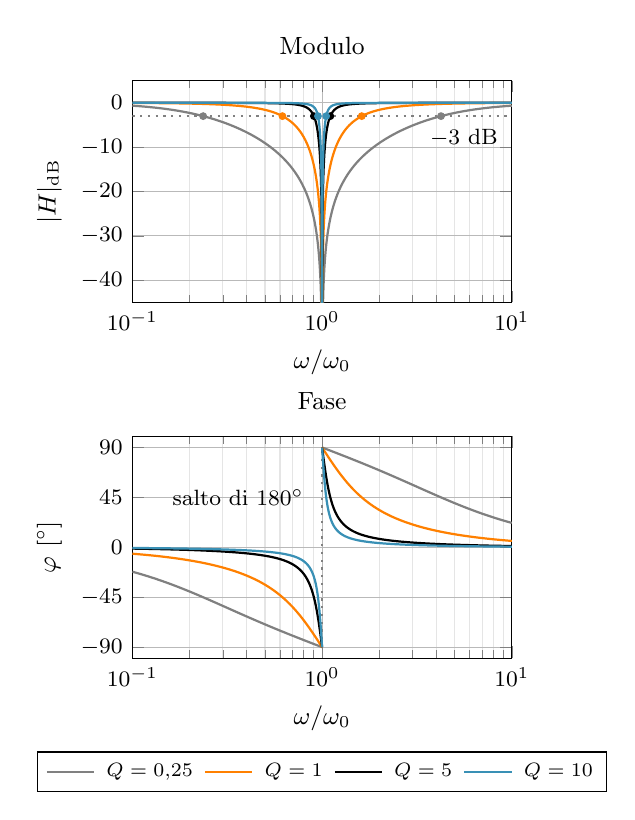
\begin{tikzpicture}
% ---------- modulo ----------
\begin{semilogxaxis}[bode mag, name=mag, xmin=0.1, xmax=10, xlabel={$\omega/\omega_0$},
  ymin=-45, ymax=5, ytick={-40,-30,-20,-10,0}]
  \addplot[gray, dotted, thick, forget plot] coordinates {(0.1,-3.01) (10,-3.01)};
  \addplot[Q025, thick, domain=-1:1, samples=1001]
    ({10^x}, {10*log10((0.25*(10^x-10^(-x)))^2/(1+(0.25*(10^x-10^(-x)))^2) + 1e-12)});
  \addplot[only marks, mark=*, mark size=1.2pt, Q025, forget plot] coordinates {(0.2361,-3.01) (4.2361,-3.01)};
  \addplot[Q1, thick, domain=-1:1, samples=1001]
    ({10^x}, {10*log10((1*(10^x-10^(-x)))^2/(1+(1*(10^x-10^(-x)))^2) + 1e-12)});
  \addplot[only marks, mark=*, mark size=1.2pt, Q1, forget plot] coordinates {(0.6180,-3.01) (1.6180,-3.01)};
  \addplot[Q5, thick, domain=-1:1, samples=1001]
    ({10^x}, {10*log10((5*(10^x-10^(-x)))^2/(1+(5*(10^x-10^(-x)))^2) + 1e-12)});
  \addplot[only marks, mark=*, mark size=1.2pt, Q5, forget plot] coordinates {(0.9050,-3.01) (1.1050,-3.01)};
  \addplot[Q10, thick, domain=-1:1, samples=1001]
    ({10^x}, {10*log10((10*(10^x-10^(-x)))^2/(1+(10*(10^x-10^(-x)))^2) + 1e-12)});
  \addplot[only marks, mark=*, mark size=1.2pt, Q10, forget plot] coordinates {(0.9512,-3.01) (1.0512,-3.01)};
  \node[anchor=north east, font=\footnotesize] at (axis cs:9.5,-3.8) {$-3$ dB};
\end{semilogxaxis}
% ---------- fase ----------
\begin{semilogxaxis}[bode fase, at={(mag.south west)}, yshift=-1.7cm, anchor=north west,
  xmin=0.1, xmax=10, xlabel={$\omega/\omega_0$},
  legend columns=4, legend style={font=\scriptsize, at={(0.5,-0.42)}, anchor=north, column sep=2pt},
  legend cell align=left]
  \addplot[gray, dotted, thick, forget plot] coordinates {(1,-90) (1,90)};
  \addplot[Q025, thick, domain=-1:-0.0001, samples=301]
    ({10^x}, {-atan2(10^x/0.25, 1-10^(2*x))});
  \addlegendentry{$Q=0{,}25$}
  \addplot[Q025, thick, forget plot, domain=0.0001:1, samples=301]
    ({10^x}, {180-atan2(10^x/0.25, 1-10^(2*x))});
  \addplot[Q1, thick, domain=-1:-0.0001, samples=301]
    ({10^x}, {-atan2(10^x/1, 1-10^(2*x))});
  \addlegendentry{$Q=1$}
  \addplot[Q1, thick, forget plot, domain=0.0001:1, samples=301]
    ({10^x}, {180-atan2(10^x/1, 1-10^(2*x))});
  \addplot[Q5, thick, domain=-1:-0.0001, samples=301]
    ({10^x}, {-atan2(10^x/5, 1-10^(2*x))});
  \addlegendentry{$Q=5$}
  \addplot[Q5, thick, forget plot, domain=0.0001:1, samples=301]
    ({10^x}, {180-atan2(10^x/5, 1-10^(2*x))});
  \addplot[Q10, thick, domain=-1:-0.0001, samples=301]
    ({10^x}, {-atan2(10^x/10, 1-10^(2*x))});
  \addlegendentry{$Q=10$}
  \addplot[Q10, thick, forget plot, domain=0.0001:1, samples=301]
    ({10^x}, {180-atan2(10^x/10, 1-10^(2*x))});
  \node[anchor=east, font=\footnotesize] at (axis cs:0.9,45) {salto di $180^\circ$};
\end{semilogxaxis}
\end{tikzpicture}
\end{document}
